\documentclass[
  bibliography=totoc,     % Literatur im Inhaltsverzeichnis
  captions=tableheading,  % Tabellenüberschriften
  titlepage=firstiscover, % Titelseite ist Deckblatt
]{scrartcl}

% Paket float verbessern
\usepackage{scrhack}

% Warnung, falls nochmal kompiliert werden muss
\usepackage[aux]{rerunfilecheck}

% unverzichtbare Mathe-Befehle
\usepackage{amsmath}
% viele Mathe-Symbole
\usepackage{amssymb}
% Erweiterungen für amsmath
\usepackage{mathtools}

% Fonteinstellungen
\usepackage{fontspec}
% Latin Modern Fonts werden automatisch geladen
% Alternativ:
%\setromanfont{Libertinus Serif}
%\setsansfont{Libertinus Sans}
%\setmonofont{Libertinus Mono}
\recalctypearea % Wenn man andere Schriftarten gesetzt hat,
% sollte man das Seiten-Layout neu berechnen lassen

% deutsche Spracheinstellungen
\usepackage{polyglossia}
\setmainlanguage{german}


\usepackage[
  math-style=ISO,    % ┐
  bold-style=ISO,    % │
  sans-style=italic, % │ ISO-Standard folgen
  nabla=upright,     % │
  partial=upright,   % ┘
  warnings-off={           % ┐
    mathtools-colon,       % │ unnötige Warnungen ausschalten
    mathtools-overbracket, % │
},                       % ┘
]{unicode-math}

% traditionelle Fonts für Mathematik
\setmathfont{Latin Modern Math}
% Alternativ:
%\setmathfont{Libertinus Math}

\setmathfont{XITS Math}[range={scr, bfscr}]
\setmathfont{XITS Math}[range={cal, bfcal}, StylisticSet=1]

% Zahlen und Einheiten
\usepackage[
locale=DE,                   % deutsche Einstellungen
separate-uncertainty=true,   % immer Fehler mit \pm
per-mode=symbol-or-fraction, % / in inline math, fraction in display math
]{siunitx}

% chemische Formeln
\usepackage[
version=4,
math-greek=default, % ┐ mit unicode-math zusammenarbeiten
text-greek=default, % ┘
]{mhchem}

% richtige Anführungszeichen
\usepackage[autostyle]{csquotes}

% schöne Brüche im Text
\usepackage{xfrac}

% Standardplatzierung für Floats einstellen
\usepackage{float}
\floatplacement{figure}{htbp}
\floatplacement{table}{htbp}

% Floats innerhalb einer Section halten
\usepackage[
section, % Floats innerhalb der Section halten
below,   % unterhalb der Section aber auf der selben Seite ist ok
]{placeins}

% Seite drehen für breite Tabellen: landscape Umgebung
\usepackage{pdflscape}

% Captions schöner machen.
\usepackage[
  labelfont=bf,        % Tabelle x: Abbildung y: ist jetzt fett
  font=small,          % Schrift etwas kleiner als Dokument
  width=0.9\textwidth, % maximale Breite einer Caption schmaler
]{caption}
% subfigure, subtable, subref
\usepackage{subcaption}

% Grafiken können eingebunden werden
\usepackage{graphicx}
% größere Variation von Dateinamen möglich
\usepackage{grffile}

% schöne Tabellen
\usepackage{booktabs}

% Verbesserungen am Schriftbild
\usepackage{microtype}

% Literaturverzeichnis
\usepackage[style=alphabetic,]{biblatex}
% Quellendatenbank
\addbibresource{lit.bib}
\addbibresource{programme.bib}

% Hyperlinks im Dokument
\usepackage[
  unicode,        % Unicode in PDF-Attributen erlauben
  pdfusetitle,    % Titel, Autoren und Datum als PDF-Attribute
  pdfcreator={},  % ┐ PDF-Attribute säubern
  pdfproducer={}, % ┘
]{hyperref}
% erweiterte Bookmarks im PDF
\usepackage{bookmark}

% Trennung von Wörtern mit Strichen
\usepackage[shortcuts]{extdash}

\title{V51: Der Operationsverstärker}
\author{
  Simon Schulte
  \texorpdfstring{
    \\
    \href{mailto:simon.schulte@udo.edu}{simon.schulte@udo.edu}
  }{}
  \texorpdfstring{\and}{, }
  Tim Sedlaczek
  \texorpdfstring{
    \\
    \href{mailto:tim.sedlaczek@udo.edu}{tim.sedlaczek@udo.edu}
  }{}
}
\publishers{TU Dortmund – Fakultät Physik}

\date{Durchführung: 11.07.2018\\
      Abgabe: 14.09.2018}


\begin{document}

\maketitle
\thispagestyle{empty}
\setcounter{page}{1}
\pagenumbering{arabic}
\section{Theorie}
\label{sec:theorie}
In diesem Versuch werden verschiedene
Schaltungen mit Hilfe des Operationsverstärkers realisiert.
Zunächst wird auf die physikalischen Eigenschaften eingegangen,
woraufhin verschiedene Schaltungen skizziert und schließlich
realisiert werden.

\subsection{Eigenschaften des Operationsverstärkers}
\label{subsec:eigenschaften}
Ein Operationsverstärker ist ein Differenzverstärker, welcher mit einem/r konstanten
Betriebsstrom/spannung gekoppelt ist.
Die wichtigste elektrische Eigenschaft des Operationsverstärkers
ist die Proportionalität der Ausgangsspannung $U_\text{A}$ zur
Differenz der Eingangsspannungen $U_\text{P}$ und $U_\text{N}$:
\begin{equation}
\label{eq:proportionalität}
    U_\text{A} = V(U_\text{P} - U_\text{N})\,,
\end{equation}
wobei $V$ die Leerlaufverstärkung bezeichnet.
Diese Beziehung gilt in einem Spannungsbereich
$-U_\text{B} < U_\text{A} < U_\text{B}$, der durch die Betriebsspannung
$U_\text{B}$ bestimmt ist. Ausserhalb dieses Bereichs läuft die
Ausgangsspannung in eine Sättigung.

\noindent
Aus dem Zusammenhang für $U_\text{A}$ ergibt sich, dass für eine positive Spannung
bei $U_\text{N}$ und $U_\text{P} \less U_\text{N}$ die Ausgangsspannung negativ wird.
Daher nennt man den negativen Eingang auch den invertierenden Eingang und den positiven
Eingang auch den nicht invertierenden.
Die Grundschaltung eines Operationsverstärkers ist in Abbildung \ref{fig:op} dargestellt.
\begin{figure}
    \centering
    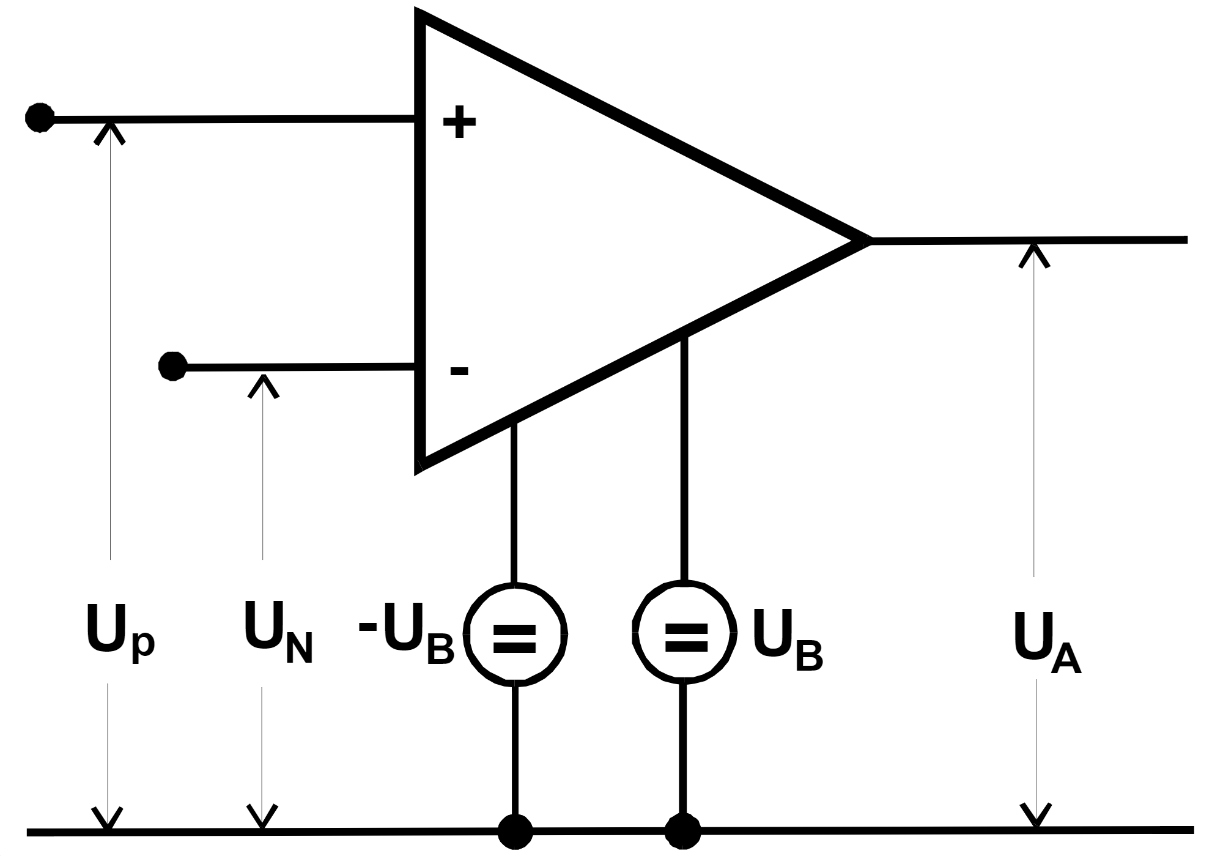
\includegraphics[width=0.5\linewidth]{op.PNG}
    \caption{
        Schaltbild eines Operationsverstärkers mit Ausgangsspannung
        $U_\text{A}$ und Eingangsspannungen $U_\text{P}$ und
        $U_\text{N}$ \cite{V51}.
    }
    \label{fig:op}
\end{figure}

\noindent
Neben der meist frequenzabhängigen Leerlaufverstärkung $V$ besitzt der
Operationsverstärker weitere Kenngrößen, wie die Eingangswiderstände,
$r_\text{e,P}$ und $r_\text{e,N}$, sowie
einen Ausgangswiderstand $r_\text{a}$.
Um Rechnungen zu Vereinfachen gilt für einen idealen Operationsverstärker
\begin{equation}
\label{eq:id-verstärker}
    V = \infty\,,\qquad r_\text{e} = \infty\,,\qquad r_\text{a} = 0\,.
\end{equation}
Aufgrund dieser Annahmen eines idealen Operationsverstärkers lassen sich die
Schaltungen mit einem Operationsverstärker relativ einfach nach Knoten- und Maschenregel
berechnen. Dabei spielt nur die äußere Beschaltung des OPVs eine Rolle.\\

\noindent
Im Gegensatz dazu müssen zur theoretischen Beschreibung eines realen
Operationsverstärkers zusätzliche Kenngrößen in Betracht gezogen werden.
\noindent
Die Gleichtaktverstärkung
\begin{equation}
\label{eq:gleichtaktverstärkung}
    V_\text{Gl} = \frac{\Delta U_\text{A}}{\Delta U_\text{Gl}}
\end{equation}
berücksichtigt geringe Asymmetrien der beiden Vertärkungskanäle.
Dabei bezeichnen $\Delta U_\text{A}$ die Differenz der Ausgangsspannung zu
\num{0} und $\Delta U_\text{Gl}$ den Unterschied der eigentlich gleichen
Eingangsspannungen.
\noindent
Die auf Grund endlicher Eingangswiderstände $r_\text{e}$ auftretenden
Eingangsströme werden mit $I_\text{P}$ und $I_\text{N}$, deren
Mittelwert,
\begin{equation}
\label{eq:eingangsruhestrom}
    I_\text{B} = \frac{1}{2}\left(I_\text{P} + I_\text{N}\right)\,,
\end{equation}
als Eingangsruhestrom und die Differenz
\begin{equation}
\label{eq:offsetstrom}
    I_0 = I_\text{P} - I_\text{N}\,,
\end{equation}
als Offsetstrom bezeichnet.
Ähnlich zum Offsetstrom, verschwindet auch die Spannung häufig nicht.
Für die Offsetspannung $U_0$ gilt daher bei $U_\text{A} = 0$
\begin{equation}
\label{eq:offsetspannung}
    U_0 = U_\text{P} - U_\text{N}\,.
\end{equation}
Sie ist abhängig von Temperatur, Zeit und Betriebsspannungen. Die totale
Ableitung wird mit Offsetspannungsdrift bezeichnet.


\section{Schaltungsbeispiele}
\label{sec:schaltungsbeispiele}
Im Folgenden werden einige Schaltbeispiele für Operationsverstärker
dargestellt.

\subsection{Arten von Operationsverstärkern}

\subsubsection{Rückgekoppelter Linearverstärker}
\label{subsubsec:rueck-linearverstärker}
Der relativ kleine Arbeitsbereich des Operationsverstärkers ist in der
Anwendung oft nicht praktikabel. Um diesen Bereich zu verbreitern, wird die
Verstärkung reduziert, indem ein Teil der Ausgangsspannung auf den
invertierenden Eingang gegeben wird. (Gegenkopplung).
Der Anteil der zurückgeführten Spannung kann dabei mit Hilfe der Widerstände
$R_1$ und $R_\text{N}$ bestimmt werden, die in Abbildung \ref{fig:linear}
dargestellt sind.
\begin{figure}[H]
    \centering
    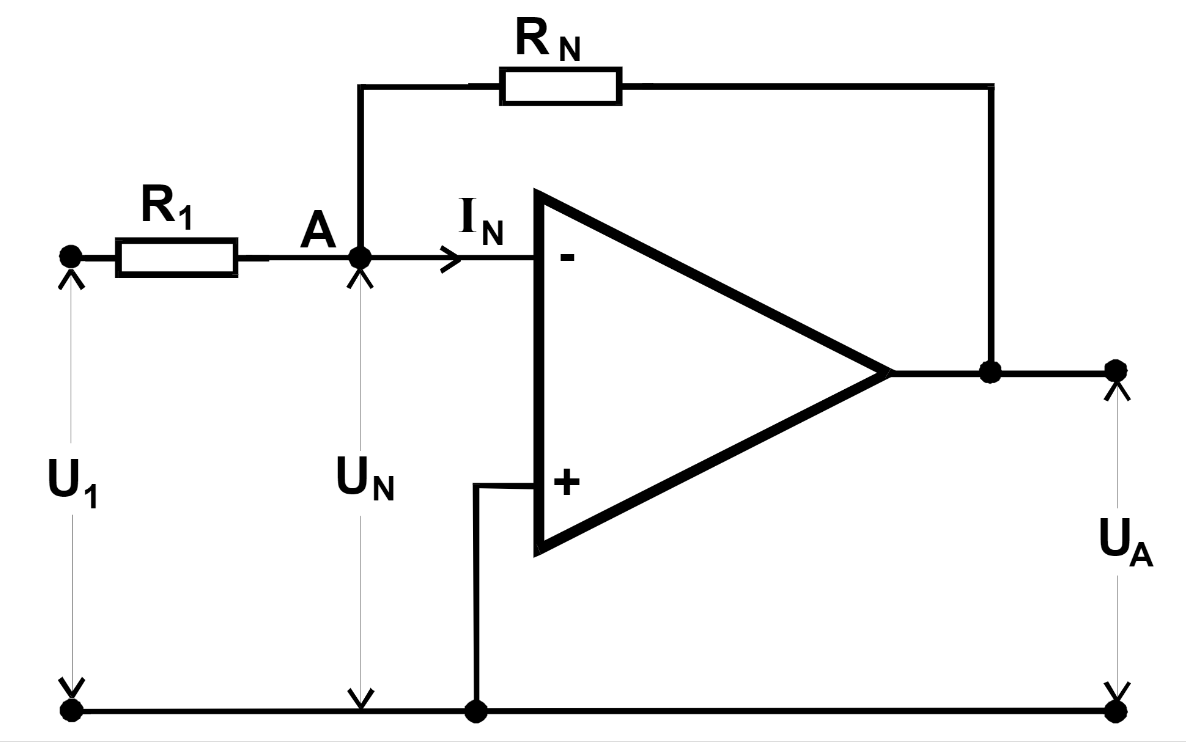
\includegraphics[width=0.5\linewidth]{linearverstaerker.PNG}
    \caption{Gegengekoppelter Linearverstärker \cite{V51}.}
    \label{fig:linear}
\end{figure}
\noindent
Bei der Annahme eines idealen Verstärkers ergibt sich über die Kirchhoffschen Regeln
ein Verstärkungsfaktor von:
\begin{equation}
  V^\prime = -\frac{R_\text{N}}{R_1}
  \label{eqn:v'lingegen}
\end{equation}
Für den Fall $R_\text{N}/R_1 \ll V$ gilt dies auch für den realen OPV.
Der Geringe Eingangswiderstand $r_\text{e} \approx R_1$ wirkt sich bei
hochohmigen Spannungsquellen möglicherweise nachteilig auf Spannungsmessungen aus.
Im nächsten Abschnitt wird daher ein Linearverstärker vorgestellt, der diesen Nachteil
umgeht.

\subsubsection{Elektrometerverstärker}
\label{subsubsec:elektrometerverstärker}
Wie in Abbildung \ref{fig:elektrometer} deutlich wird, wird auch bei diesem
Verstärker ein Teil der Ausgangsspannung $U_\text{A}$ zum invertierenden
Eingang zurückgeführt. Dabei sind die Widerstände $R_1$ und $R_\text{N}$ auf
eine andere Art und Weise verschaltet, sodass der Eingangswiderstand in der
Größenordnung des Gleichtakteingangwiderstandes
($r_\text{Gl} \approx \SI{10}{\giga\ohm}$) liegt, hier tritt das eventuelle
Problem des zu geringen Eingangswiderstandes also nicht auf.
Stattdessen kann hier ein Eingangsruhestrom $I_\text{B}$ für Probleme sorgen,
indem er am Innenwiederstand einer Spannungsquelle einen Spannungsabfall hervorruft.
Die Verstärkung $V^\prime$ des Elektrometerverstärkers beträgt
\begin{equation*}
    V^\prime = \frac{U_\text{A}}{U_1} = \frac{R_\text{N} + R_1}{R_1}\,.
\end{equation*}
\begin{figure}[H]
    \centering
    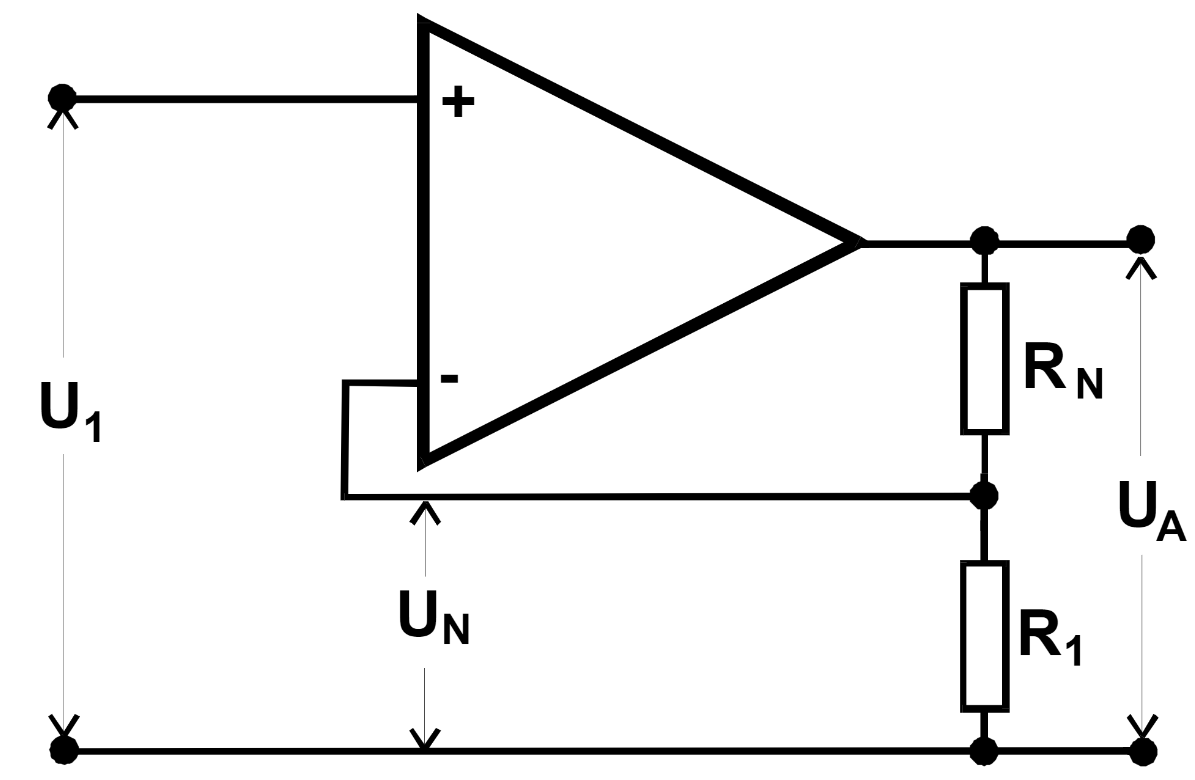
\includegraphics[width=0.5\linewidth]{elektrometer.PNG}
    \caption{Schaltbild eines Elektrometerverstärkers \cite{V51}.}
    \label{fig:elektrometer}
\end{figure}

\subsubsection{OP mit geringem Eingangswiderstand $R_\text{e}$ (Ampèremeter)}
\label{subsubsec:amperemeter}
Im Gegensatz zum grossen Eingangswiderstand $R_\text{e}$ eines
Elektrometerverstärkers lässt sich, wie in Abbildung
\ref{fig:amperemeter} dargestellt, ein Linearverstärker mit
besonders geringem Eingangswiderstand konstruieren.
Somit können zum Beispiel Ströme in einem Ampèremeter gemessen werden, wobei
der dazu nötige Spannungsabfall $\Delta U$ besonders gering ist.
\begin{figure}[H]
    \centering
    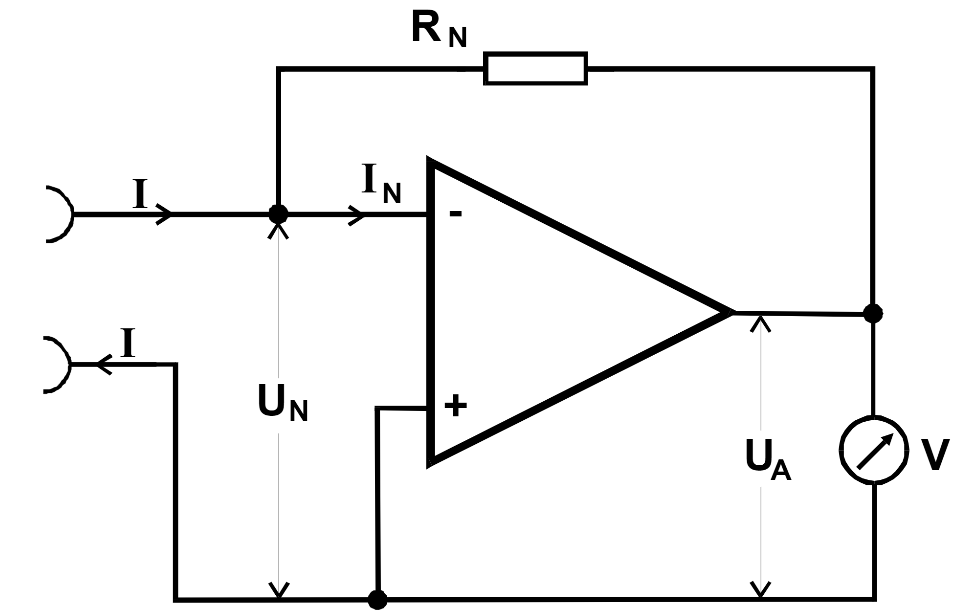
\includegraphics[width=0.5\linewidth]{amperemeter.png}
    \caption{Schaltbild eines Elektrometerverstärkers \cite{V51}.}
    \label{fig:amperemeter}
\end{figure}

\subsection{Umkehr-Integrator und -Differentiator}
\label{subsec:integrator}
Mit Hilfe eines zusätzlichen Kondensators mit Kapazität $C$ in der Schaltung
eines Linearverstärkers lässt sich entweder ein Integrations- oder eine
Differentiationsglied bauen.
Für die Ausgangsspannungen $U_\text{A,I}$ des Integrators und $U_\text{A,D}$
des Differentiators gilt dann
\begin{align*}
    U_\text{A,I} &= - \frac{1}{RC} \int U_1\!(t) \mathup{d}t\,,\\
    \text{und} \qquad U_\text{A,D} &= - RC \frac{\mathup{d}U_1}{\mathup{d}t}\,.
\end{align*}
Dabei bezeichnet $R$ den Widerstand.
Integrator und Differentiator besitzen also Tief- und Hochpass Eigenschaften und
unterscheiden sich nur durch die Positionen des Widerstandes und des Kondensators.
Die entsprechenden Schaltungen sind in Abbildung \ref{fig:integrator} dargestellt.
\begin{figure}[H]
    \begin{subfigure}{.49\linewidth}
        \centering
        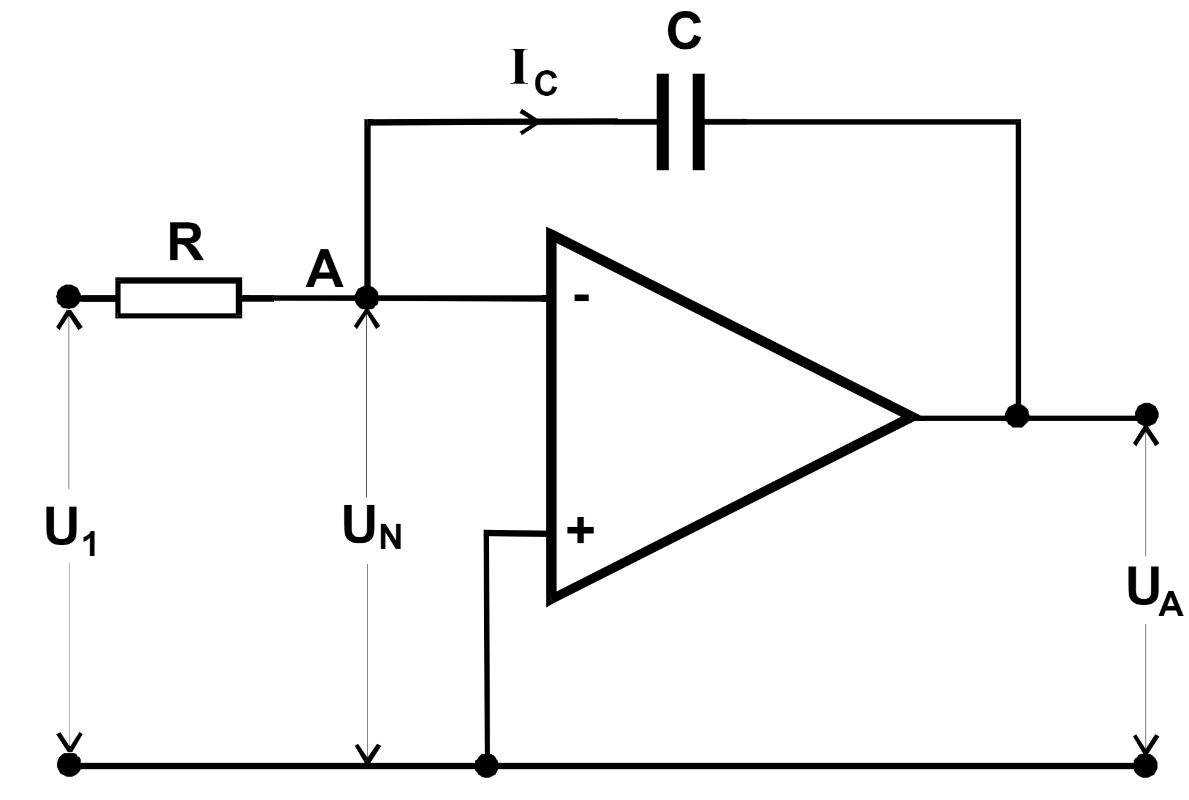
\includegraphics[width=1.0\linewidth]{integrator.PNG}
        \caption{Schaltbild eines Umkehr-Integrators \cite{V51}.}
        \label{fig:integrator-integrator}
    \end{subfigure}
    \begin{subfigure}{.49\linewidth}
        \centering
        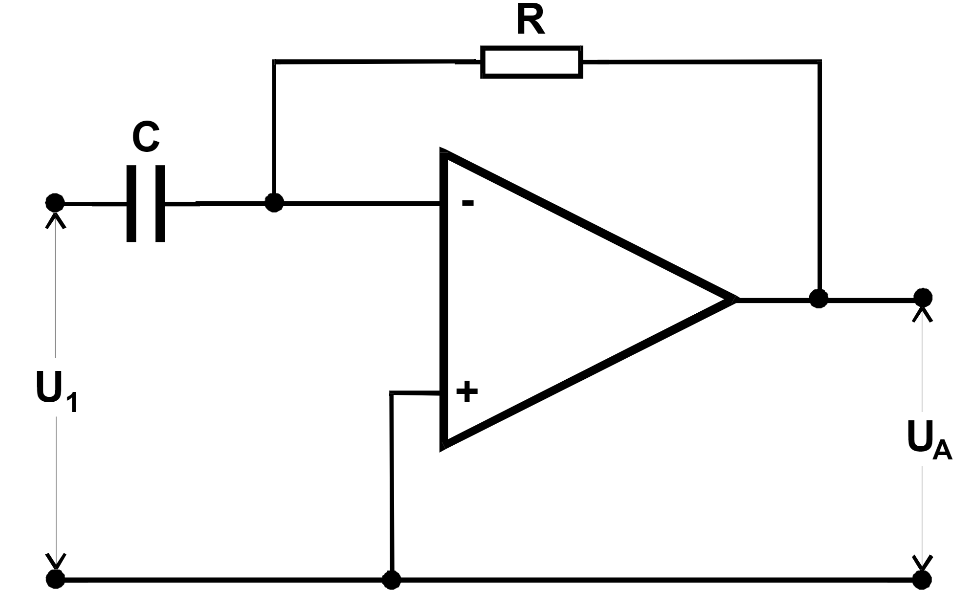
\includegraphics[width=1.0\linewidth]{differentiator.PNG}
        \caption{Schaltbild eines Umkehr-Differentiators \cite{V51}.}
        \label{fig:integrator-differentiator}
    \end{subfigure}
    \caption{Linearverstärker mit Kondensator.}
    \label{fig:integrator}
\end{figure}

\subsection{Logarithmierer und Exponentialgenerator}
\label{subsec:log_expo}
Neben Differential- und Integral-Operationen können auch Exponentierung nud
Logarithmierung mit Hilfe des Operationsverstärkers umgesetzt werden.
Dabei wird statt eines Kondensators eine Diode eingebaut.
Dabei gilt für die entsprechenden Ausgangssignale $U_\text{A,E}$ und
$U_\text{A,L}$
\begin{align*}
    U_\text{A,L} &= R I_0 \exp\left(\frac{e_0}{k_\text{B}T} U_\text{e}\right)\,,\\
    \text{und} \qquad U_\text{A,E} &= \frac{k_\text{B}T}{e_0}\ln \frac{U_\text{e}}{R I_0}\,,
\end{align*}
mit der absoluten Temperatur $T$, der Boltzmannkonstante $k_\text{B}$ und
der Elementarladung $e_0$. Abbildung \ref{fig:log_expo} zeigt die Schaltungen.
\begin{figure}[H]
    \begin{subfigure}{.49\linewidth}
        \centering
        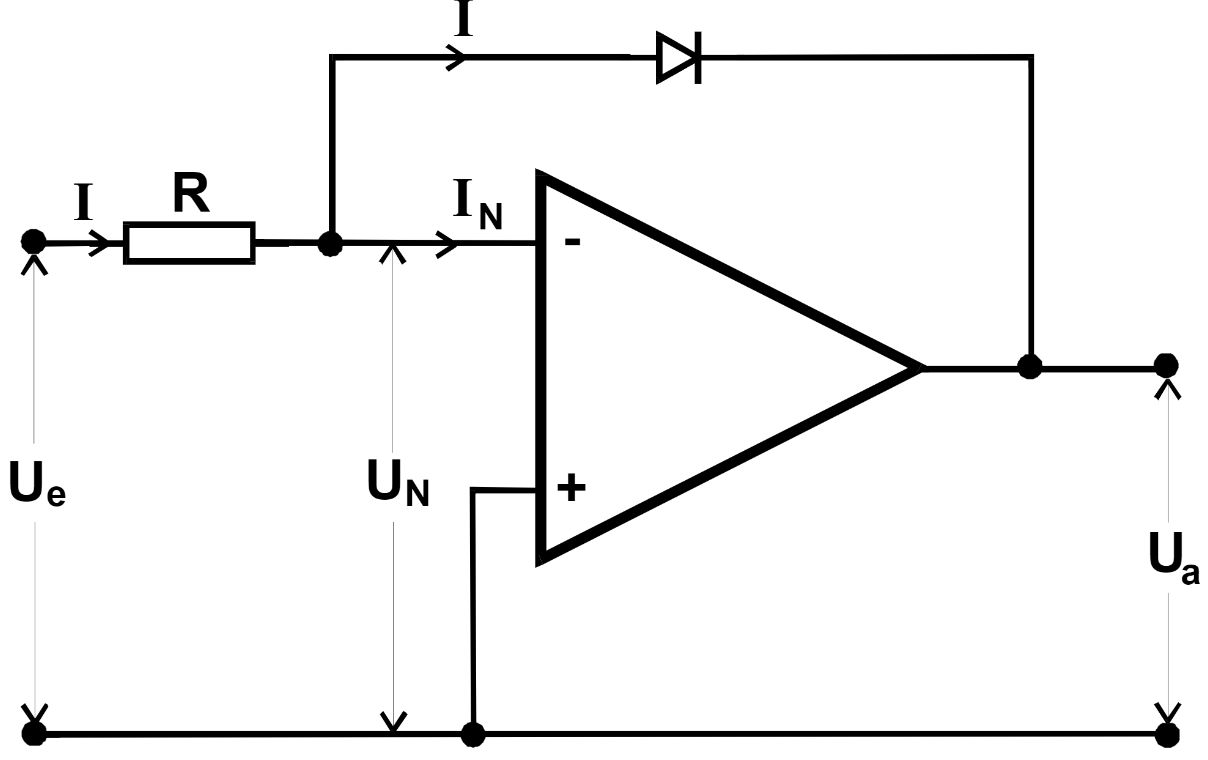
\includegraphics[width=1.0\linewidth]{log.PNG}
        \caption{Schaltbild eines Logarithmierers \cite{V51}.}
        \label{fig:log}
    \end{subfigure}
    \begin{subfigure}{.49\linewidth}
        \centering
        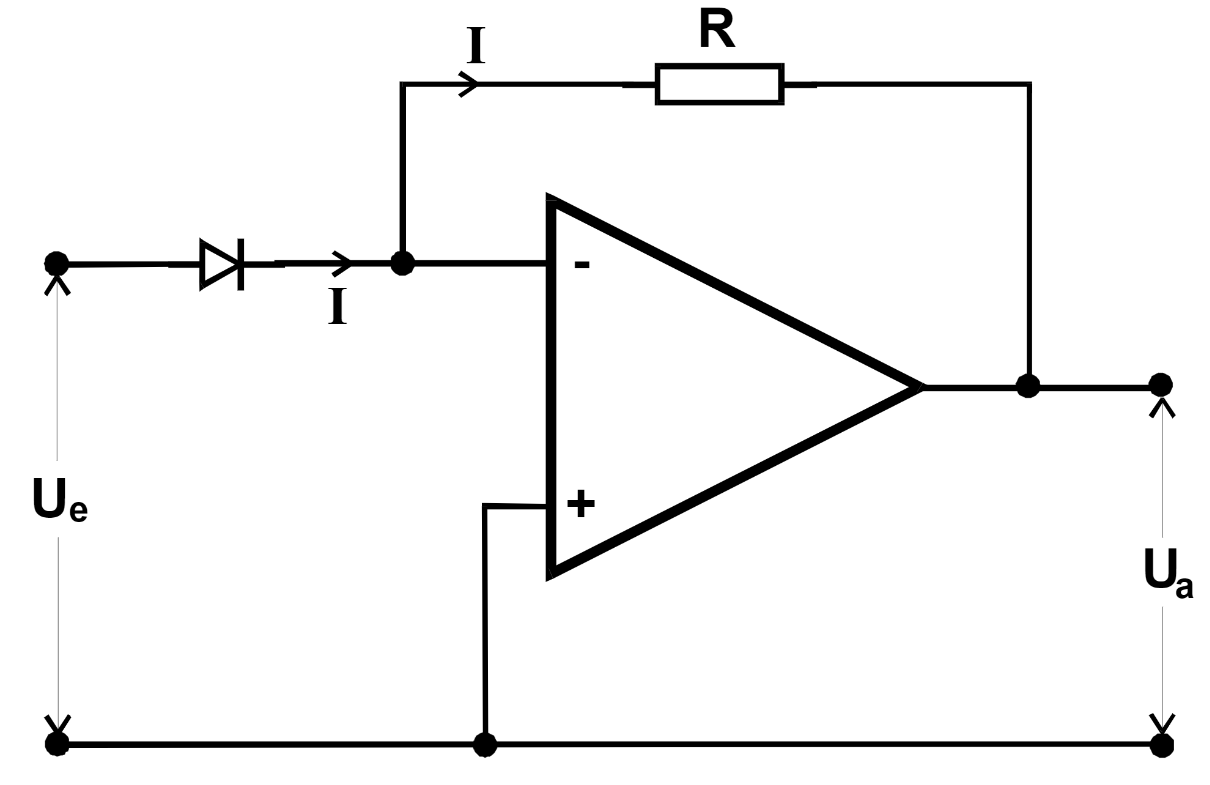
\includegraphics[width=1.0\linewidth]{expo.PNG}
        \caption{Schaltbild eines Exponentialgenerators \cite{V51}.}
        \label{fig:expo}
    \end{subfigure}
    \caption{Linearverstärker mit Diode.}
    \label{fig:log_expo}
\end{figure}

\subsection{Schmitt-Trigger}
\label{subsec:schmitt_trigger}
Der Operationsverstärker kann als Schalter genutzt werden. Statt, wie bisher
einen Teil der Ausgangsspannung auf invertierenden Eingang zu geben (Gegenkopplung),
wird dieser Anteil auf den nicht-invertierenden Eingang gegeben (Mitkopplung).
Damit wird das eigene Ausgangssignal verstärkt und der Operationsverstärker erreicht
schnell die Sättigungsspannung $U_\text{B}$.
\begin{align}
    U_\text{A} =
    \begin{cases}
        +U_\text{B} &: U_1 > \frac{R_1}{R_\text{P}}U_\text{B} \\
        -U_\text{B} &: U_1 < -\frac{R_1}{R_\text{P}}U_\text{B}\,,
    \end{cases}
    \label{eqn:schmitt}
\end{align}
mit der Betriebsspannugn $U_\text{B}$. Der Schmitt-Trigger besitzt also im Gegensatz
zu anderen Schaltern nicht nur eine Schaltschwelle, sondern zwei: Eine obere Einschaltschwelle
und eine untere Abschaltschwelle. Mit dieser Eigenschaft eignet sich der Schmitt-Trigger
besonders gut zur bereinigung von digitalen Signalen.
Die entsprechende Schaltung ist in Abbildung \ref{fig:schmitt_trigger}
dargestellt.
\begin{figure}[H]
    \centering
    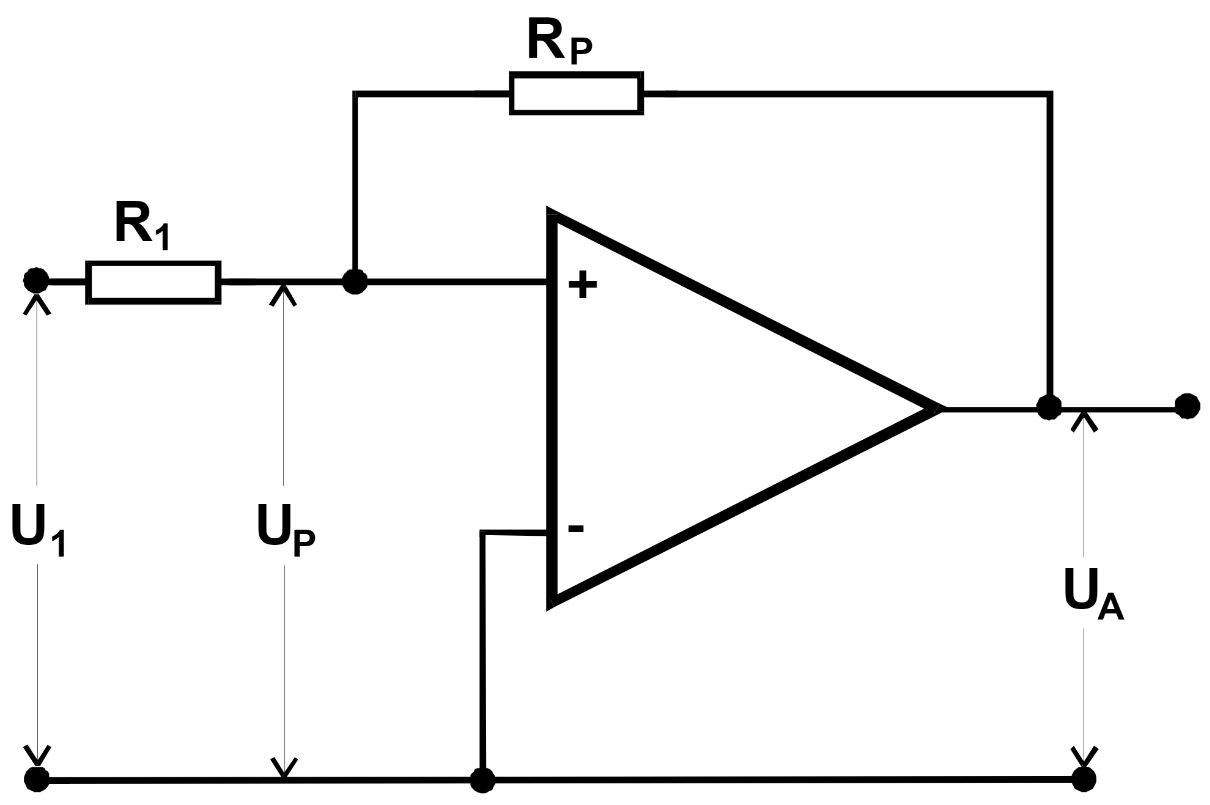
\includegraphics[width=0.5\linewidth]{schmitt_trigger.PNG}
    \caption{
        Schaltbild eines Operationsverstärkers, der als Schmitt-Trigger
        genutzt wird.
    }
    \label{fig:schmitt_trigger}
\end{figure}
\clearpage
\subsection{Signalgenerator}
\label{subsec:signalgenerator}
Schließlich können mit Hilfe eines Operationsverstärkers verschiedene
Signalspannungen erzeugt werden. Dazu wird jeweils eine Mehrzahl von OPVs
miteinander verschaltet.

\subsubsection{Erzeugung von Dreieck- und Rechteckspannungen}
\label{subsubsec:dreieck}
Durch Kombination eines Schmitt-Triggers mit einem Integrationsglied
lassen sich Dreiecks- und Rechtecksspannungen erzeugen. Damit wird die
Integration genutzt, um den Schmitt-Trigger zu schalten und somit das
Vorzeichen des Signals zu ändern. Je nach Ausgang der in Abbildung
\ref{fig:dreieck} dargestellten Schaltung erhält man die gewünschte
Spannungsform.
\begin{figure}[H]
    \centering
    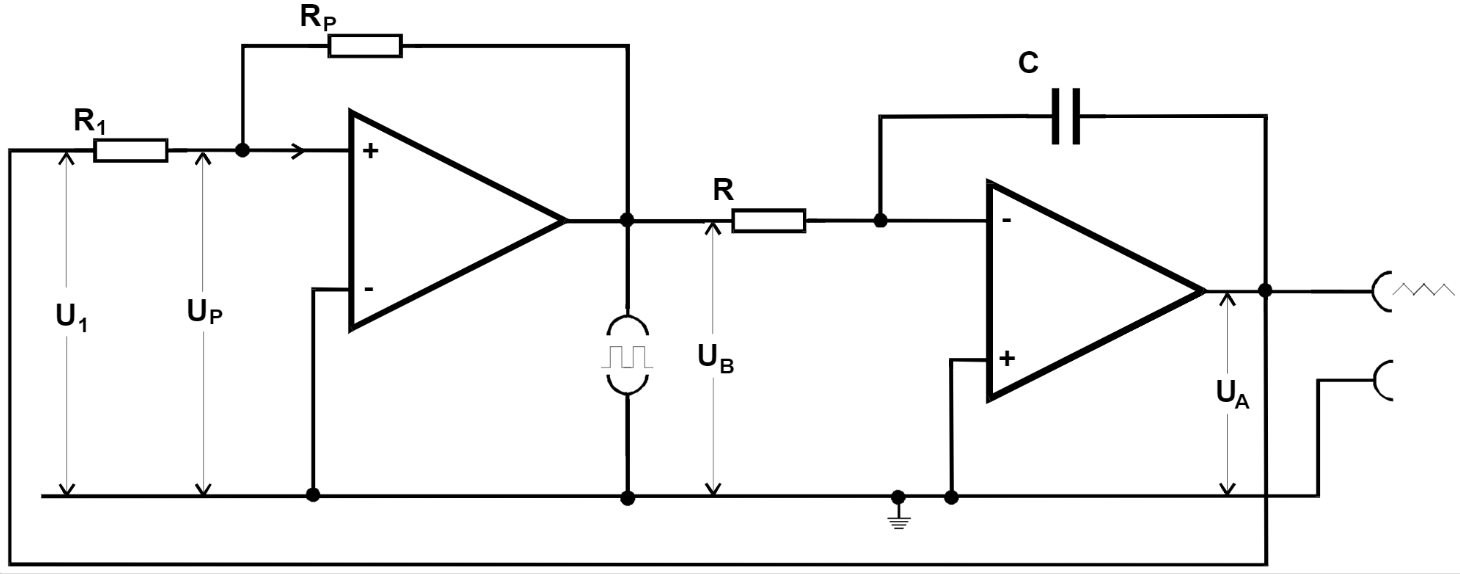
\includegraphics[width=0.9\linewidth]{dreieck.PNG}
    \caption{
        Schaltbild zur Erzeugung von Dreieck- und Recheckspannungen:
        Es wird ein OP als Integrationsglied mit einem Schmitt-Trigger
        verschaltet \cite{V51}.
    }
    \label{fig:dreieck}
\end{figure}

\subsubsection{Erzeugung von Sinusschwingungen}
\label{subsubsec:sinusschwingungen}
Durch Kombination zweier Integratoren mit einem Umkehrverstärker lassen sich
gedämpfte Sinusschwingungen erzeugen.
Die Schaltung kann durch eine Differentialgleichung 2. Ordung beschrieben
werden und liefert die Lösung
\begin{equation}
    U_\text{A}(t) = U_0 \exp\!\left( \frac{\eta t}{\num{20} RC} \right)
                        \sin\!\left( \frac{t}{RC} \right)\,.
    \label{eqn:oszi}
\end{equation}
Dabei ist $\num{-1} < \eta < \num{1}$ durch das Potentiometer $P$ einzustellen.
Die Schwingungsdauer beträgt dabei $T = 2\pi RC$, die Abklingzeit
$\tau = 20 RC / |\eta|$. Damit sollte die Amplitude für $\eta = \num{0}$
konstant bleiben.
Das Schaltbild zu einem Sinusgenerator ist in Abbildung \ref{fig:sinus}
dargestellt.
\begin{figure}[H]
    \centering
    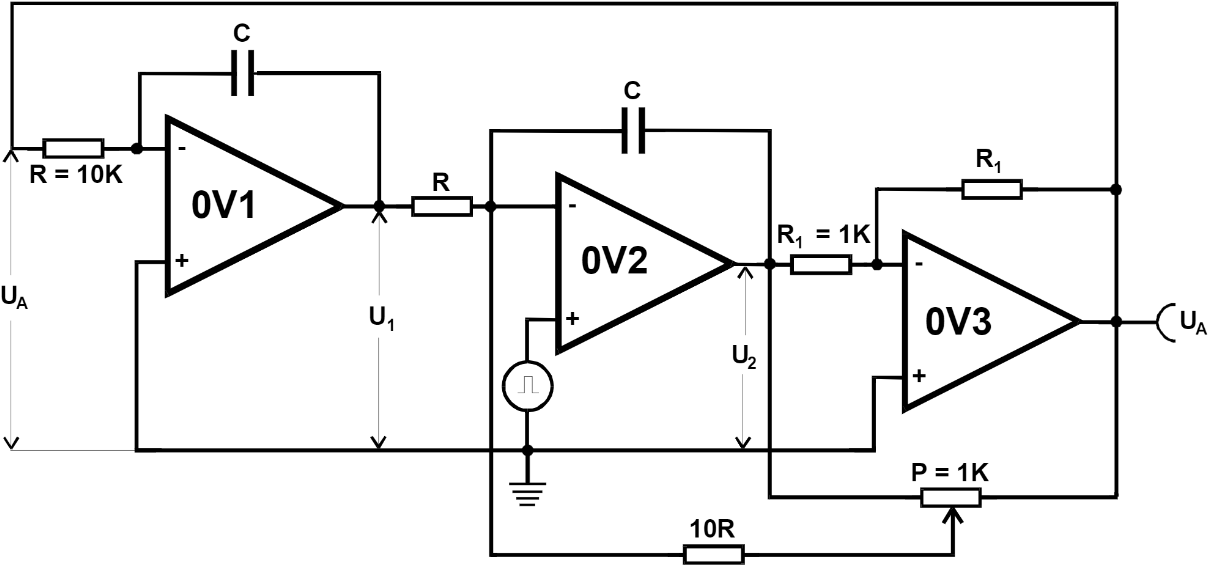
\includegraphics[width=0.9\linewidth]{sinus.PNG}
    \caption{
        Schaltbild eines Sinusgenerators. Es werden zwei Integrationsglieder
        und ein Umkehrverstärker verbaut \cite{V51}.
    }
    \label{fig:sinus}
\end{figure}

\section{Durchführung}
\label{sec:durchführung}
%[16:36, 9.7.2018] tim s: ADEFH


Mit Hilfe der Schaltung \ref{fig:linear} wird zunächst der Frequenzgang eines
gegengekoppelten Verstärkers bei vier verschiedenen Verstärkungsgraden $V'$
und über mehrere Zehnerpotenzen untersucht. \\
\\
\noindent
Als nächstes wird ein Umkehr-Integrator \ref{fig:integrator-integrator} zur Überprüfung der Beziehung
$U_a \approx \frac{1}{\nu}$ (der Tiefpass Eigenschaft) aufgebaut. Außerdem werden
verschiedene Signalformen eines Funktionsgenerators auf den Integrator gegeben und
die Ausgangssignale an einem Oszilloskop beobachtet. \\
\\
\noindent
Daraufhin wird ein Umkehr-Differentiator nach Schaltung \ref{fig:integrator-differentiator} verwendet
und wie beim Umkehr-Integrator verfahren. \\
\\
\noindent
Danach wird ein Schmitt-Trigger wie in Abbildung \ref{fig:schmitt_trigger} aufgebaut.
Auf den Eingang wird ein Sinus-Signal gegeben. Das Ausgangssignal wird erneut an einem
Oszilloskop beobachtet und die Spannungsschwelle vermessen. \\
\\
\noindent
Als Letztes werden gedämpfte Schwingungen untersucht. Zur Realisierung einer gedämpften
Schwingung wird die Schaltung nach Abbildung \ref{fig:sinus} verwendet. Zur Erzeugung
der Schwingung wird vor dem OPV 2 ein Rechteckgenerator mit eingebaut. An einem
Potentiometer wird dann $\eta = -1$ für eine gedämpfte Schwingung eingestellt.
\clearpage
\section{Auswertung}
\label{sec:auswertung}
\subsection{Fehlerrechnung}
Für die Fehlerrechnung sowie den mathematischen Teil der Auswertung wird auf
$\textsc{Python}$ zurückgegriffen:\\
Regressionen sowie deren Fehler wurden durch die $\textsc{Numpy}$ \cite{numpy} Funktion
$\textsc{curve-fit}$ durchgeführt. Grafiken wurden mit $\textsc{Matplotlib}$ \cite{matplotlib}
erstellt.
Fehlerfortpflanzung wird durch die Bibliothek
$\textsc{Uncertainties}$ \cite{uncertainties} automatisiert.

\subsection{Gegengekoppelter Linearverstärker}
Bei dem gegengekoppelter Linearverstärker werden die Werte aus Tabelle \ref{tab:messwerte1}
gemessen. Die Graphen dazu sind in den Abbildungen \ref{fig:plot} bis \ref{fig:plot4}
zu sehen. Für die maximal gemessene Ausgangsspannung wird jeweils der Wert
$\frac{V^\prime}{\sqrt{2}}$ berechnet und als Konstante eingezeichnet. Die Bandbreite
ist bis zu dem Schnittpunkt der beiden Kurven definiert. Die Grenzfrequenz $\nu^\prime_g$
wird and den Graphen abgelesen bzw. mit den Messwerten abgeschätzt.
Sie stehen zusammen mit den Widerstandsverhältinssen der einzelnen Schaltungen in Tabelle \ref{tab:widver}.
Außerdem ist in der Tabelle das Verstärkungs-Bandbreite-Produkt aufgelistet .
\begin{table}[H]
  \centering
  \caption{Die Widerstandsverhältnisse der Schaltungen.}
  \label{tab:widver}
  \begin{tabular}{c c c c}
    \toprule
    Schaltung & Widerstandverhältnis & Grenzfrequenz & V-B-Produkt \\
    \midrule
    1 & $V^\prime = \SI{469}{\ohm}/\SI{468}{\ohm} \approx 1$        & $\nu^\prime_g \approx \SI{1150}{\kilo\hertz}$ & $\nu^\prime_g \cdot V^\prime \approx \SI{1152}{\kilo\hertz}$ \\
    2 & $V^\prime = \SI{996}{\ohm}/\SI{468}{\ohm} \approx 2$        & $\nu^\prime_g \approx \SI{775}{\kilo\hertz}$  & $\nu^\prime_g \cdot V^\prime \approx \SI{1649}{\kilo\hertz}$ \\
    3 & $V^\prime = \SI{10}{\kilo\ohm}/\SI{468}{\ohm} \approx 21$   & $\nu^\prime_g \approx \SI{112}{\kilo\hertz}$  & $\nu^\prime_g \cdot V^\prime \approx \SI{2393}{\kilo\hertz}$ \\
    4 & $V^\prime = \SI{33.1}{\kilo\ohm}/\SI{468}{\ohm} \approx 71$ & $\nu^\prime_g \approx \SI{40}{\kilo\hertz}$   & $\nu^\prime_g \cdot V^\prime \approx \SI{2829}{\kilo\hertz}$ \\
    \bottomrule
  \end{tabular}
\end{table}
\begin{table}
  \centering
  \caption{Die gemessenen Spannungen für den gegengekoppelten Linearverstärker.}
  \label{tab:messwerte1}
  \begin{tabular}{c c c c c c c c}
    \toprule
    \multicolumn{2}{c}{Schaltung: 1} & \multicolumn{2}{c}{2} & \multicolumn{2}{c}{3} & \multicolumn{2}{c}{4} \\
    $\nu$ in $\si{\hertz}$ & $U_\text{A}$ in $\si{\milli\volt}$ & $\nu$ in $\si{\hertz}$ & $U_\text{A}$ in $\si{\milli\volt}$ & $\nu$ in $\si{\hertz}$ & $U_\text{A}$ in $\si{\milli\volt}$ & $\nu$ in $\si{\hertz}$ & $U_\text{A}$ in $\si{\milli\volt}$ \\
    \midrule
    0.4   & 259.5 & 0.4  & 255.5 & 0.4  & 255.5 & 0.4  & 245   \\
    16.4  & 259.5 & 20   & 255.5 & 16.4 & 251.5 & 16.4 & 225   \\
    32.4  & 259.5 & 40   & 255.5 & 32.4 & 239   & 32.4 & 183   \\
    48.35 & 259.5 & 80   & 254.5 & 48.4 & 230   & 48.4 & 148.5 \\
    64.35 & 259.5 & 120  & 248   & 66.4 & 213   & 64   & 120.5 \\
    80.3  & 259.5 & 160  & 251   & 82.4 & 203   & 80   & 103.5 \\
    96.3  & 259.5 & 200  & 243   & 96.4 & 191   & 96   & 88.5  \\
    112   & 259.5 & 240  & 239   & 112  & 181   & 112  & 78.5  \\
    128   & 258   & 280  & 234   & 128  & 167   & 128  & 72.5  \\
    144   & 256.5 & 320  & 234   & 144  & 155   & 144  & 64.5  \\
    160   & 256.5 & 360  & 223   & 160  & 146.5 & 160  & 60.5  \\
    176   & 256.5 & 400  & 221   & 176  & 136.5 & 176  & 55.5  \\
    192   & 256.5 & 500  & 211   & 192  & 128.5 & 192  & 53.5  \\
    208   & 256.5 & 550  & 207   & 208  & 121.5 & 208  & 48    \\
    224   & 255   & 600  & 200   & 224  & 116.5 & 224  & 45    \\
    240   & 255   & 650  & 195   & 240  & 109.5 & 240  & 44    \\
    256   & 255   & 700  & 187   & 256  & 104.5 & 256  & 40    \\
    272   & 252   & 750  & 183   & 272  & 99.5  & 272  & 39    \\
    288   & 252   & 800  & 177   & 288  & 94.5  & 288  & 39    \\
    304   & 250.5 & 850  & 170   & 304  & 90.5  & 304  & 36    \\
    320   & 250.5 & 900  & 165   & 320  & 88.5  & 320  & 34    \\
    336   & 249   & 950  & 161   & 336  & 84.5  & 336  & 32    \\
    352   & 249   & 1000 & 156   & 352  & 80.5  & 352  & 32    \\
    368   & 244.5 &      &       & 368  & 76.5  & 368  & 32    \\
    384   & 244.5 &      &       & 384  & 76.5  & 384  & 32    \\
    400   & 244.5 &      &       & 400  & 72.5  & 400  & 32    \\
    1181  & 182   &      &       &      &       &      &       \\
    1750  & 143.5 &      &       &      &       &      &       \\
    1930  & 136   &      &       &      &       &      &       \\
    1000  & 195.5 &      &       &      &       &      &       \\
    900   & 204.5 &      &       &      &       &      &       \\
    800   & 211   &      &       &      &       &      &       \\
    2000  & 133   &      &       &      &       &      &       \\
    \bottomrule
  \end{tabular}
\end{table}
\begin{figure}
  \centering
  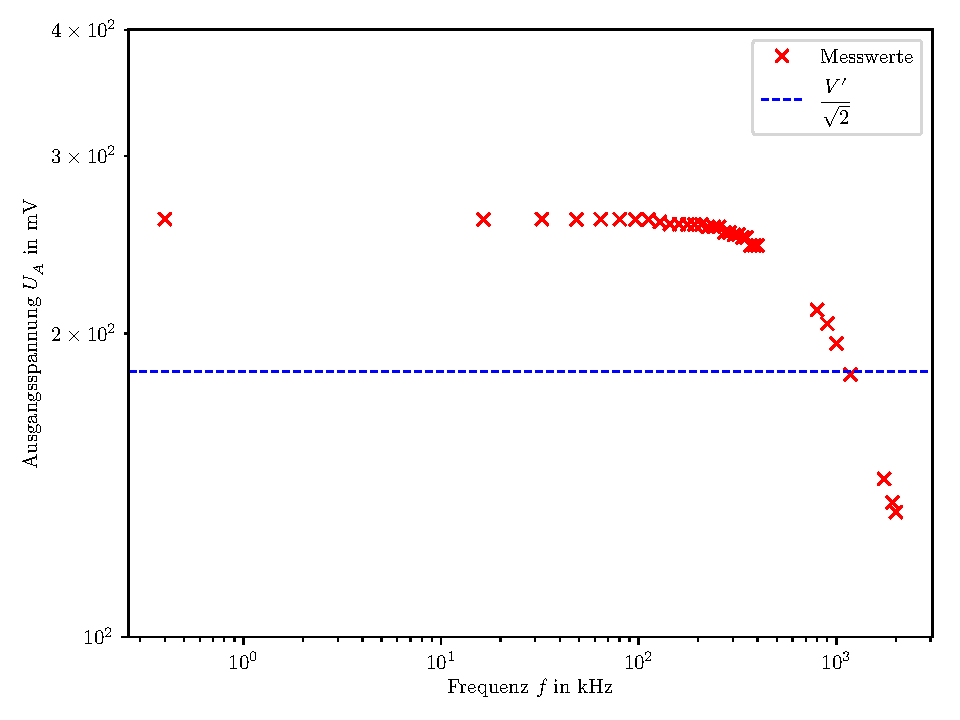
\includegraphics[width=0.8\textwidth]{plot.pdf}
  \caption{Messwerte mit Schaltung 1.}
  \label{fig:plot}
\end{figure}
\begin{figure}
  \centering
  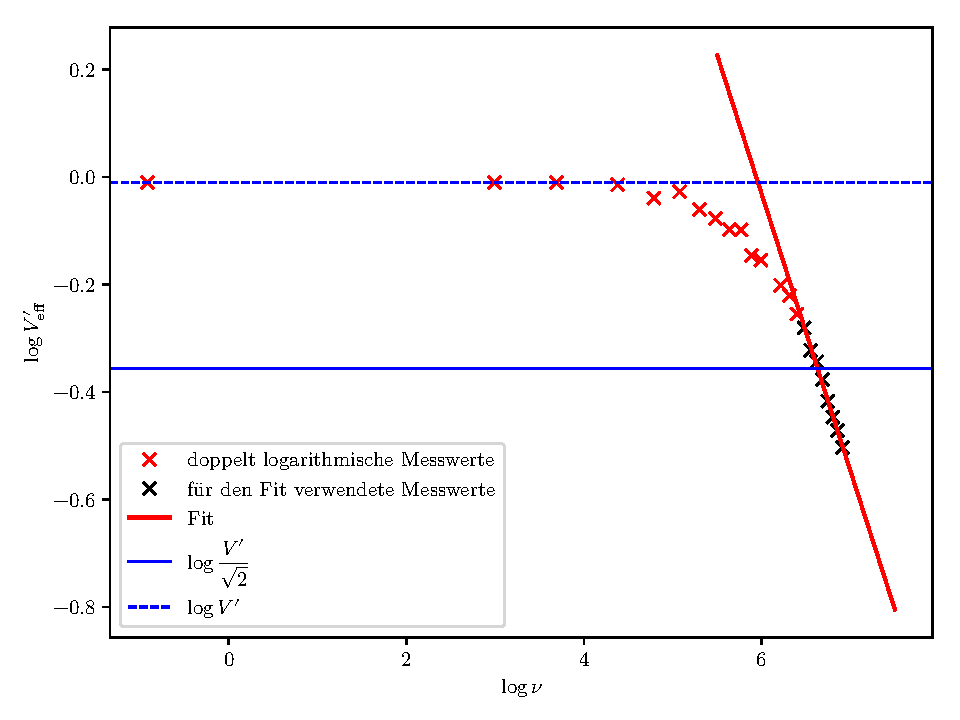
\includegraphics[width=0.8\textwidth]{plot2.pdf}
  \caption{Messwerte mit Schaltung 2.}
  \label{fig:plot2}
\end{figure}
\begin{figure}
  \centering
  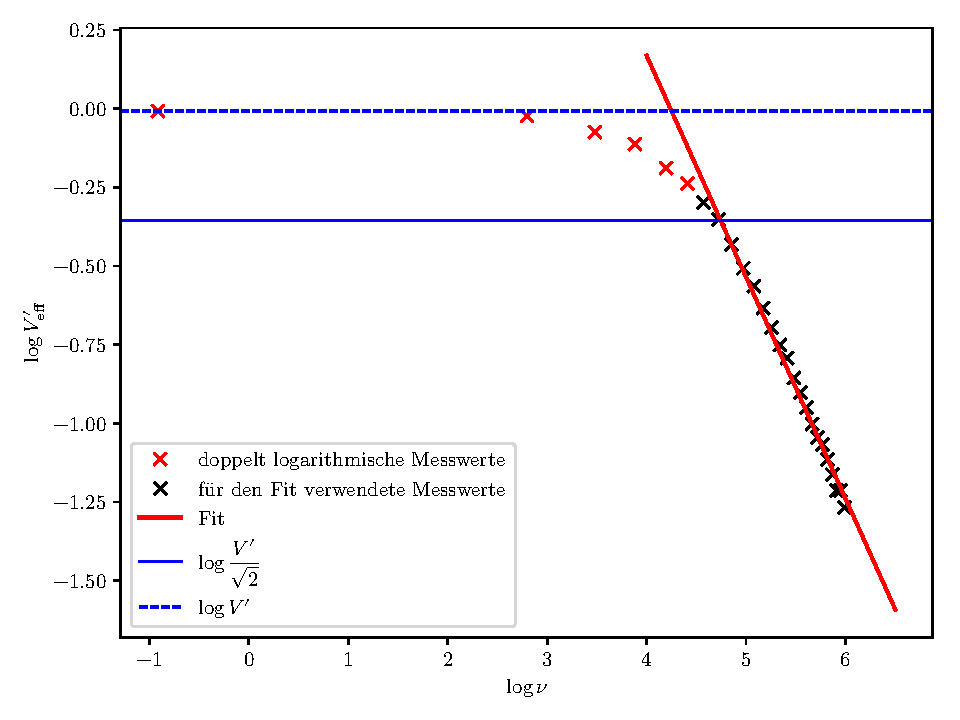
\includegraphics[width=0.8\textwidth]{plot3.pdf}
  \caption{Messwerte mit Schaltung 3.}
  \label{fig:plot3}
\end{figure}
\begin{figure}
  \centering
  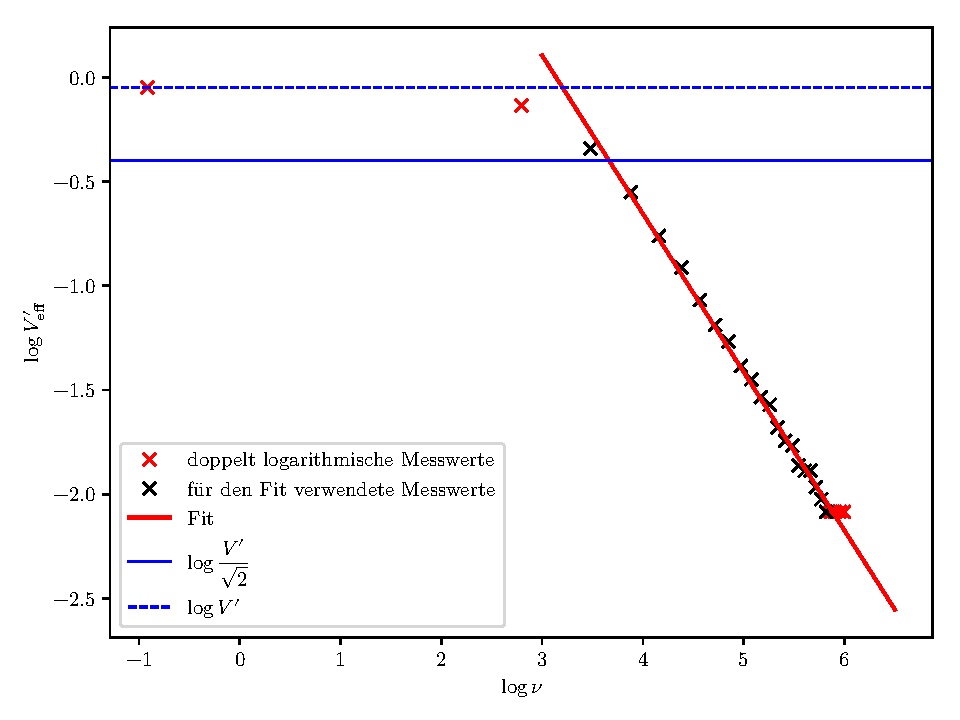
\includegraphics[width=0.8\textwidth]{plot4.pdf}
  \caption{Messwerte mit Schaltung 4.}
  \label{fig:plot4}
\end{figure}
\clearpage

\subsection{Differentiator und Integrator}
Diese beiden Schaltungen haben aufgrund eines technischen Defektes nicht funktioniert.
In dem Signal waren unschöne ungewollte Schwingungen zu sehen, die aussahen wie die
bei einer Fouriertransformierten. Dadurch war eine Aufnahme des Frequenzverhaltens unmöglich.

\subsection{Schmitt-Trigger}
In Abbildung \ref{fig:schmitttrigg} ist eine Bildschirmaufnahme des Eingangs- und
des Ausgangssignals des Schmitt-Triggers zu sehen. Dabei ist das grüne Signal das Eingangssignal
und das gelbe Signal das Ausgangssignal.
\begin{figure}[H]
  \centering
  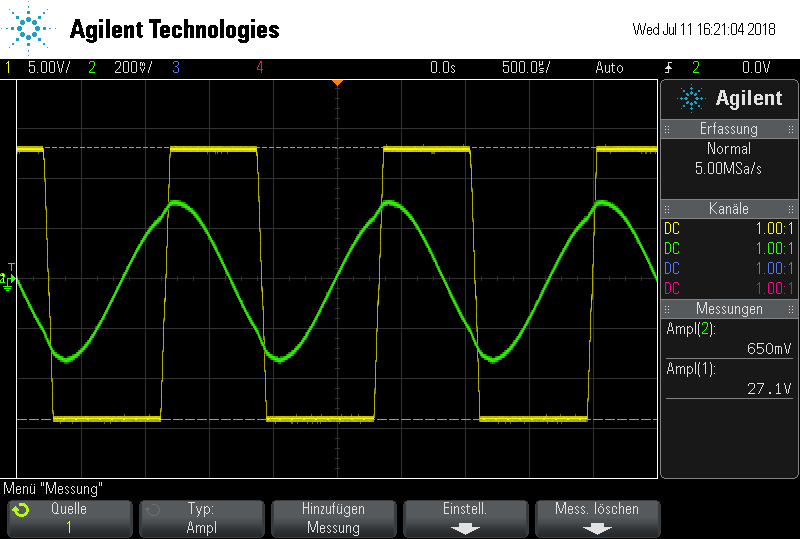
\includegraphics[width=0.8\textwidth]{schmitt.png}
  \caption{Bildschirmaufnahme Schmitt-Trigger.}
  \label{fig:schmitttrigg}
\end{figure}
\noindent
Die gemessenen Scheitelspannungen sind:
\begin{align*}
  U_\text{e,ein} &= \SI{278(5)}{\milli\volt} \\
  U_\text{e,aus} &= \SI{-249(5)}{\milli\volt}.
\end{align*}
Als Ausgangsspannung werden
\begin{align*}
  U_\text{B} &= \SI{13.0(1)}{\volt} \\
  -U_\text{B} &= \SI{-14.0(1)}{\volt}
\end{align*}
gemessen und die verwendeten Widerstände betragen:
\begin{align*}
  R_1 &= \SI{470(4)}{\ohm} \\
  R_\text{P} &= \SI{33.1(2)}{\kilo\ohm}.
\end{align*}
Mit diesen Werten ergeben sich nach den Formeln \eqref{eqn:schmitt} theoretische
Werte für die Scheitelspannungen:
\begin{align*}
  U_\text{e,ein} &= \SI{199(3)}{\volt} \\
  U_\text{e,aus} &= \SI{-185(2)}{\volt}.
\end{align*}

\subsection{Oszillator Schaltung}
Für diese Schaltung war aus dem gleichen Grund, wie bei den Differentiator- und
Integratorschaltungen, keine Messung möglich. Die Werte haben wir daher
von dem Betreuer erhalten. Sie sind in Abbildung \ref{fig:plot5} dargestellt.
\begin{figure}[H]
  \centering
  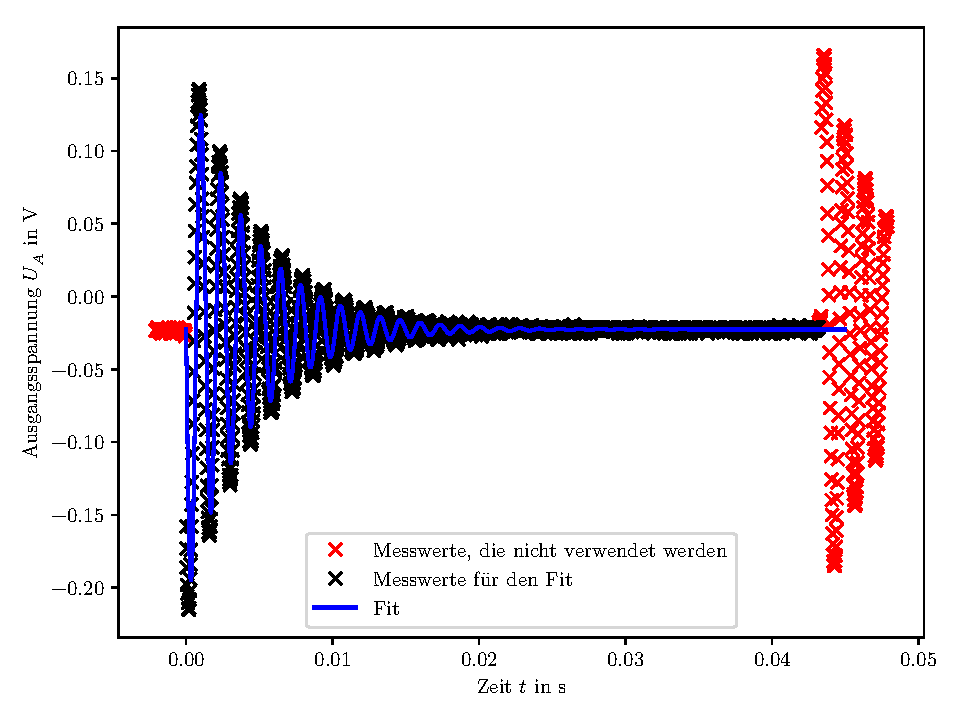
\includegraphics[width=0.8\textwidth]{plot5.pdf}
  \caption{Werte und Fit zu der Oszillator Schaltung.}
  \label{fig:plot5}
\end{figure}
\noindent
Es werden alle Werte aussortiert, die vor der ersten Anregung und nach der zweiten
Anregung durch die Rechteckspannung liegen. Die restlichen Werte werden anschließend
nach einer Funktion
\begin{equation*}
  f(t) = a \cdot \exp{\left(\frac{bt}{20 \cdot c}\right)} \cdot \sin{\left(\frac{t}{c}\right)} + d
\end{equation*}
gefittet.
Als Startwerte für den Fit dienen dabei:
\begin{align*}
  a &= \SI{200}{\milli\volt} \\
  b &= \SI{-1}{} \\
  c &= \SI{224}{\nano\second} \\
  d &= \SI{-20}{\milli\volt}.
\end{align*}
Bei dem Fit ergeben sich folgende Parameter:
\begin{align*}
  a &= \SI{186(4)}{\milli\volt} \\
  b &= \SI{-1.00(3)}{} \\
  c &= \SI{216.5(2)}{\nano\second} \\
  d &= \SI{-22.6(4)}{\milli\volt}.
\end{align*}
Die verwendeten Bauteile haben die Werte:
\begin{align*}
  R &= \SI{9.96}{\kilo\ohm} \\
  C_1 &= \SI{21.5}{\nano\farad} \\
  C_2 &= \SI{23.6}{\nano\farad} \\
  10R &= \SI{99.6}{\kilo\ohm} \\
  R_1 &= \SI{996}{\ohm}
\end{align*}
Da die Werte der Kapazitäten eine etwas größere Differenz besitzen, werden diese
beiden Werte gemittelt. Der Mittelwert ist: $C = \SI{22.6(10)}{\nano\farad}$.
Damit wird jetzt der Theoriewert für die Konstante $c$ des Fits berechnet.
Nach Formel \eqref{eqn:oszi} folgt:
\begin{equation*}
  c = R \cdot C = \SI{225(10)}{\nano\second}.
\end{equation*}

\section{Diskussion}
\label{diskussion}
Auffällig ist, dass bei den gegengekoppelten Linearverstärkerschaltungen die
maximale Ausgangsspannung immer gleich war und etwa der Eingangsspannung entsprach.
Außerdem ist das Verstärkung-Bandbreite-Produkt nicht konstant. Das erste
Problem (möglicherweise damit auch das Zweite) ließ sich am Ende dadurch lösen,
dass man den Widerstand, welcher zu dem OPV parallel geschaltet wird, "direkt"
in die Schaltung auf dem Entwicklerboard einbaut und nicht "indirekt"
über Verkabelungen anschließt. Dadurch hat die Schmitt-Trigger Schaltung später
gut Funktioniert. Allerdings war die Zeit zu knapp um die ersten Messreihen zu
wiederholen. Die Differentiator- und Integratorschaltungen haben leider aus genannten
Gründen nicht funktioniert. Der Schmitt-Trigger hat gut funktioniert und seine
Aufgabe erfüllt. Die Scheitelspannungen liegen allerdings etwas höher als erwartet.
Eventuell sind dafür die unter der idealen Annahme vernachlässigten Eigenschaften
eines realen OPVs verantwortlich oder es hing ebenfalls mit dem defekten Entwicklerboard
zusammen. Die Daten zu der Oszillatorschaltung verhalten sich weitestgehend wie
erwartet. Bei dem Fit ergeben sich sinnvolle Werte, die mit den Theoriewerten übereinstimmen.
\newpage
\nocite{*}
\printbibliography

\end{document}
